\documentclass{article}

% if you need to pass options to natbib, use, e.g.:
% \PassOptionsToPackage{numbers, compress}{natbib}
% before loading nips_2018

% ready for submission
\usepackage[preprint]{nips_2018}

% to compile a preprint version, e.g., for submission to arXiv, add
% add the [preprint] option:
% \usepackage[preprint]{nips_2018}

% to compile a camera-ready version, add the [final] option, e.g.:
% \usepackage[final]{nips_2018}

% to avoid loading the natbib package, add option nonatbib:
% \usepackage[nonatbib]{nips_2018}

\usepackage[utf8]{inputenc} % allow utf-8 input
\usepackage[T1]{fontenc}    % use 8-bit T1 fonts
\usepackage{hyperref}       % hyperlinks
\usepackage{url}            % simple URL typesetting
\usepackage{booktabs}       % professional-quality tables
\usepackage{amsfonts}       % blackboard math symbols
\usepackage{nicefrac}       % compact symbols for 1/2, etc.
\usepackage{microtype}      % microtypography
\usepackage{macros}   %user custom packages

\title{A Gadget Problem for Medical Applications}

% The \author macro works with any number of authors. There are two
% commands used to separate the names and addresses of multiple
% authors: \And and \AND.
%
% Using \And between authors leaves it to LaTeX to determine where to
% break the lines. Using \AND forces a line break at that point. So,
% if LaTeX puts 3 of 4 authors names on the first line, and the last
% on the second line, try using \AND instead of \And before the third
% author name.

\author{
  Subhojyoti Mukherjee\thanks{Use footnote for providing further
    information about author (webpage, alternative
    address)---\emph{not} for acknowledging funding agencies.} \\
  College of Information and Computer Science\\
  University of Massachusetts Amherst\\
  Massachusetts, MA 01003 \\
  \texttt{http://bio-nlp.org/index.php/people} \\
  %% examples of more authors
  %% \And
  %% Coauthor \\
  %% Affiliation \\
  %% Address \\
  %% \texttt{email} \\
  %% \AND
  %% Coauthor \\
  %% Affiliation \\
  %% Address \\
  %% \texttt{email} \\
  %% \And
  %% Coauthor \\
  %% Affiliation \\
  %% Address \\
  %% \texttt{email} \\
  %% \And
  %% Coauthor \\
  %% Affiliation \\
  %% Address \\
  %% \texttt{email} \\
}

\begin{document}
% \nipsfinalcopy is no longer used

\maketitle

%\begin{abstract}
%To be written.
%\end{abstract}

%\keywords{Changepoint, UCB1, UCB-Improved, Regret}

\section{Introduction}
\label{review:intro}
In this report we build a gadget world  for the Reinforcement Learning (RL) setup for the medical domain. A gadget problem is a simple environment which captures some of the complexities of the real-world domain which we are trying  to model. We can test various RL algorithms in this gadget worlds before transitioning to the real-world higher complexity environments. The hypothesis behind creating such gadget worlds is that if an RL algorithms performs poorly in this small gadget world, it will surely perform poorly in real-world domains.

\section{Some complexities of Medical Domain}
\label{review:complexity}
Some of the difficult features that constitute the medical domain which we try to model in this gadget world are :-

\begin{itemize}
\item The medical environment is a partially observed environment. At any instant the physician is only exposed to some of the factors influencing the health of the patient.
\item Long horizon problem where you only receive the feedback at the end of the episode or the feedbacks are very sparse in nature.
\item Time constrained treatment, which requires that the effective treatment needs to be delivered within a fixed time otherwise it may result in death.
\item Time varying adversarial feedbacks, which may be encountered in sudden spikes in responses from the patient to the treatments administered.
\end{itemize}


\section{Notations, Assumptions and Definitions}
\label{review:notations}
We use capitalized calligraphic notations to denote sets while individual elements within the set is denoted by non-capitalized alphabets. The random variables are denoted by capitalized, non-calligraphic alphabets. $\A$ denotes the finite set of actions  with individual action indexed by $A_t = a$ such that action taken at time $t$ is $a$. We assume that the total number of actions is constant throughout the time horizon. We assume that the transition function is stationary that is, it is not changing between episodes.

%$T$ denotes the time horizon. We use capitalized calligraphic notations to denote sets while individual elements within the set is denoted by non-capitalized alphabets. $\A$ denotes the finite set of actions  with individual action indexed by $a$ such that $a=1,\ldots, K$. We assume that the total number of actions is discrete and constant throughout the time horizon and $|\A|=K$. In the gridworld setting $K=4$. We define an MDP $M$ with the tuple $M  = (\S,\A,P,d_R, d_0,\gamma)$ where $\S$ is the set of states, $\A$ is the set of actions, $P$ is the transition function, $d_R$ is the reward distribution over the states indicating how the rewards are generated, $d_0$ is the initial state distribution and $\gamma$ is the discounting factor.

\section{MDP Formulation}
\label{review:mdp}


A RL setting is usually characterized by a MDP or Markov Decision Process. A MDP is defined by the tuple $\lbrace \S,\A, P, d_R, d_{0},\gamma\rbrace$ where each element of the tuple is defined as:-
\begin{enumerate}
\item $\S$ is the finite state space such that at each time step $t$ the patient is in state $S_t \in \S$. This state space can be discrete or continuous depending on the modeling assumption of the learner.
\item $\A$ is the action space such that at each time t, the agent takes
action $\A_t \in \A$, which causes it to change its state from $S_t$ to $S_{t+1}$. Again this action space can be discrete or continuous depending on the modeling assumption of the learner.
\item $P$ is the transition function which describes how the state of the environment changes. So, $P(s,a,s') = Pr(S_{t+1}=s' | S_{t} = s, A_{t} = a)$
\item $d_R$ denotes the process of reward generation when the state of the agent changes.
\item $d_0$ denotes the initial state distribution of the agent.
\item The discount factor, $\gamma$, determines the relative weight of immediate and long-term rewards. 
\end{enumerate}

The goal of the RL agent is to learn a policy, i.e. a mapping $\pi : \S \times \A \rightarrow [0,1]$  from states to actions, that maximizes the expected discounted return $G_t$

\begin{align*}
J(\pi) &= \mathbb{E}[\sum_{t=0}^{\infty}G_t | \pi] = \mathbb{E}[\sum_{t=0}^{\infty}\gamma^t R_t | \pi]
\end{align*}

where $R_t$ is all the accumulated rewards by the agent and $T$ denotes the time horizon. 

%$T$ denotes the time horizon. We use capitalized calligraphic notations to denote sets while individual elements within the set is denoted by non-capitalized alphabets. $\A$ denotes the finite set of actions  with individual action indexed by $a$ such that $a=1,\ldots, K$. We assume that the total number of actions is constant throughout the time horizon and $|\A|=K$. The state of an 




\section{Experiments}
\label{review:expt}
\subsection{Toy Gridworld Domain}

In this section, we run Q-learning and Sarsa with linear function approximation in the two gridworld domain shown in Figure \ref{fig:gridworld1} and Figure \ref{fig:gridworld2}. The results of the experiments are shown in Figure \ref{fig:1} and Figure \ref{fig:2} for the domain 1 and 2 respectively. All the algorithms were averaged over $50$ independent trials and each trial consisted of $6000$ episodes.

\textbf{Experiment 1 (Domain 1):} In this experiment we use linear function approximation for both Q-Learning and Sarsa to handle this partially observed environment. From Figure \ref{fig:1} we see that Sarsa performs better than Q-Learning in this Domain and stabilizes before Q-Learning.

\textbf{Experiment 2 (Domain 2):} In this experiment again we use linear function approximation for both Q-Learning and Sarsa to handle this partially observed environment. From Figure \ref{fig:2} we see that Sarsa performs worse than Q-Learning in this Domain. Infact both the algorithms does not stabilize in this experiment. This results from the fact the the entry to the state $S_t = G$ is restricted and both the algorithms spend considerable amount of time in fruitless exploration.


\begin{figure}[!th]
    \begin{center}
    \begin{tabular}{cc}
    \setlength{\tabcolsep}{0.1pt}
    \subfigure[2.75\textwidth][Expt-$1$: $10\times 10$ Gridworld (Domain 1)]
    %with $r_{i_{{i}\neq {*}}}=0.07$ and $r^{*}=0.1$
    {
    		\pgfplotsset{
		tick label style={font=\large},
		label style={font=\large},
		legend style={font=\large},
		ylabel style={yshift=12pt},
		%legend style={legendshift=32pt},
		}
        \begin{tikzpicture}[scale=0.8]
      	\begin{axis}[
		xlabel={Episodes},
		ylabel={Discounted Return},
		grid=major,
        %clip mode=individual,grid,grid style={gray!30},
        clip=true,
        %clip mode=individual,grid,grid style={gray!30},
  		legend style={at={(0.5,1.4)},anchor=north, legend columns=3} ]
      	% UCB
		\addplot table{results/NewExpt/Expt1/comp_subsampled_QlearningA.txt};
		\addplot table{results/NewExpt/Expt1/comp_subsampled_SarsaA.txt};
		\addplot table{results/NewExpt/Expt1/comp_subsampled_QlearningL.txt};
		\addplot table{results/NewExpt/Expt1/comp_subsampled_SarsaL.txt};
      	\legend{Q-Learning, Sarsa, Q($\lambda$), Sarsa($\lambda$)}   
      	\end{axis}
      	\end{tikzpicture}
  		\label{fig:1}
    }
    &
    \subfigure[2.75\textwidth][Expt-$2$: $10\times 10$ Gridworld (Domain 2)] 
    %with $r_{i_{{i}\neq {*}}}=0.07$ and $r^{*}=0.1$
    {
    		\pgfplotsset{
		tick label style={font=\large},
		label style={font=\large},
		legend style={font=\large},
		ylabel style={yshift=12pt},
		%legend style={legendshift=32pt},
		}
        \begin{tikzpicture}[scale=0.8]
      	\begin{axis}[
		xlabel={Episodes},
		ylabel={Discounted Return},
		grid=major,
        %clip mode=individual,grid,grid style={gray!30},
        clip=true,
        %clip mode=individual,grid,grid style={gray!30},
  		legend style={at={(0.5,1.4)},anchor=north, legend columns=3} ]
      	% UCB
		\addplot table{results/NewExpt/Expt2/comp_subsampled_QlearningA.txt};
		\addplot table{results/NewExpt/Expt2/comp_subsampled_SarsaA.txt};
		\addplot table{results/NewExpt/Expt2/comp_subsampled_QlearningL.txt};
		\addplot table{results/NewExpt/Expt2/comp_subsampled_SarsaL.txt};
      	\legend{Q-Learning, Sarsa, Q($\lambda$), Sarsa($\lambda$)}   	
      	\end{axis}
      	\end{tikzpicture}
  		\label{fig:2}
    }
    \end{tabular}
    \end{center}
    \caption{A comparison of the performance of various algorithms. }
    \label{fig:algoExpt}
    \vspace*{-1em}
\end{figure}

\subsection{Classic Domain}

The mountain car was first described in Andrew Moore's Thesis \citep{Efficient memory-based learning for robot control} and was latter properly defined in \citet{DBLP:journals/ml/SinghS96}. The task consist of driving a car resting in a valley up the mountain. The main challenge of this task is that the car by itself cannot drive up the mountain and it has to swing back and forth to gather the sufficient momentum to reach the top of the mountain (see Figure \ref{fig:3}). Nonetheless, this simple environment consist of several challenges that afflicts the medical domain. It's a continuous state space problem, hence function approximation has to be used which makes it a partially observed MDP. Moreover, the car can only accumulate a positive reward of $+50$ when it reaches the top or suffers a negative reward of $-1$ the time while it swings back and forth.  So this models the long horizon problem. The action space is discrete in this toy domain. 

In Figure \ref{fig:4} we show how Q($\lambda$) and Sarsa($\lambda$) along with Fourier basis can be used to solve this problem.

\begin{figure}[!th]
    \begin{center}
    \begin{tabular}{cc}
    \setlength{\tabcolsep}{0.1pt}
    \subfigure[2.75\textwidth][Domain-$3$: Mountain Car]
    %with $r_{i_{{i}\neq {*}}}=0.07$ and $r^{*}=0.1$
    {
    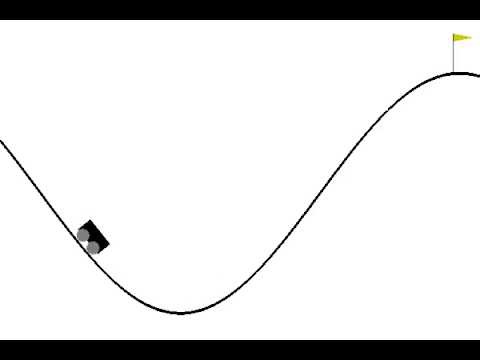
\includegraphics[scale=0.35]{img/mountain_car.jpeg}
    \label{fig:3}
    }
    \setlength{\tabcolsep}{0.1pt}
    \subfigure[2.75\textwidth][Expt-$3$: Mountain Car]
    %with $r_{i_{{i}\neq {*}}}=0.07$ and $r^{*}=0.1$
    {
    		\pgfplotsset{
		tick label style={font=\large},
		label style={font=\large},
		legend style={font=\large},
		ylabel style={yshift=12pt},
		%legend style={legendshift=32pt},
		}
        \begin{tikzpicture}[scale=0.8]
      	\begin{axis}[
		xlabel={Episodes},
		ylabel={Discounted Return},
		grid=major,
        %clip mode=individual,grid,grid style={gray!30},
        clip=true,
        %clip mode=individual,grid,grid style={gray!30},
  		legend style={at={(0.5,1.4)},anchor=north, legend columns=3} ]
      	% UCB
		\addplot table{results/NewExpt/Expt3/comp_subsampled_Qlearning.txt};
		\addplot table{results/NewExpt/Expt3/comp_subsampled_Sarsa.txt};
		\addplot table{results/NewExpt/Expt3/comp_subsampled_Qlearning1.txt};
		\addplot table{results/NewExpt/Expt3/comp_subsampled_Sarsa1.txt};
      	\legend{Q-Learning, Sarsa, Q($\lambda$), Sarsa($\lambda$)}   
      	\end{axis}
      	\end{tikzpicture}
  		\label{fig:4}
    }
    \end{tabular}
    \end{center}
    \caption{A comparison of the performance of various algorithms. }
    \label{fig:algoExpt1}
    \vspace*{-1em}
\end{figure}



\section{Conclusions and Future Works}
\label{review:conc}
In this report we formulated two gadget domains which are easy to handle and yet has sufficient complexities to handle many important and intriguing features of the real-life medical domain. We also showed that both Q-Learning and Sarsa with linear approximation fails to perform well in these domains. Future work includes proposing new algorithm that might perform better in these environments or to test planning algorithms in these domains.

%\clearpage
%\newpage


\bibliographystyle{apalike}
\bibliography{biblio1}

\end{document}
